\begin{abstract}
An OFDM structure from modulator to demodulator is studied. The aim is to investigate the characteristics of the system in different conditions and comparing the behavior with the single carrier configuration. The simulation conditions change in the cyclic prefix size, a Non-Linear Amplifier (NLA), multipath and equalizer activation. \\ Optimization on the cost function for the system is done. Semi-Analysis calculation for noise for a target Bit Error Rate (BER) of $10^{-3}$ are done. OFDM simulation is based on the characteristic of Fast Fourier Transform.\\
The analysis shows that using a multipath increases the needed \textit{energy per bit to noise power spectral density ratio} $(E_{b}/N_{0})$ by $13dB$ in order to reach the target BER when the NLA block is deactivated. An equalization block improves by $8dB$ the $(E_{b}/N_{0})$. In comparison, the multipath, more than the guard time of the signal, does not influence the BER so much.\\ With activated NLA with fixed $\beta=10$ the $E_{b}/N_{0}$ has to be amplified by almost $0.8dB$ in order to reach the target BER. \\ The optimized back-off of $\beta=8$ improves this value by $14dB$ when equalization block is activated.
 
\end{abstract}

\section{Introduction}
An OFDM communication system is simulated. Different characteristics of the system are examined and parameters are adjusted to study.\\ A block based signaling configuration is chosen for the implementation. As a result, the realization of the modulator is done thanks to IFFT computation characteristics. Cyclic prefixes are added to the resulting OFDM symbols as well as guard time filling. On the demodulator an FFT block recreates the initial input of the system. \\
An optimization is performed on the input back-off of a Non-Linear Amplifier (NLA). The back-off of the NLA is normally more than in a single carrier system because of better performance of the inter symbol interference (ISI) thanks to smaller coherent bandwidth which let us work on less power. \\
A description of the the system is given in section \ref{sec_systemmodel}. Section \ref{sec_simstruct} describes the varied parameters and analysis values while in section \ref{sec_anasim} observations on the simulation are presented and characteristics of the system are shown. Before the conclusion in section \ref{sec_conclusion}, section \ref{sec_optimization} describes the optimization of the system.

\section{System Model}
\label{sec_systemmodel}
\begin{figure}[tbp]
\centering
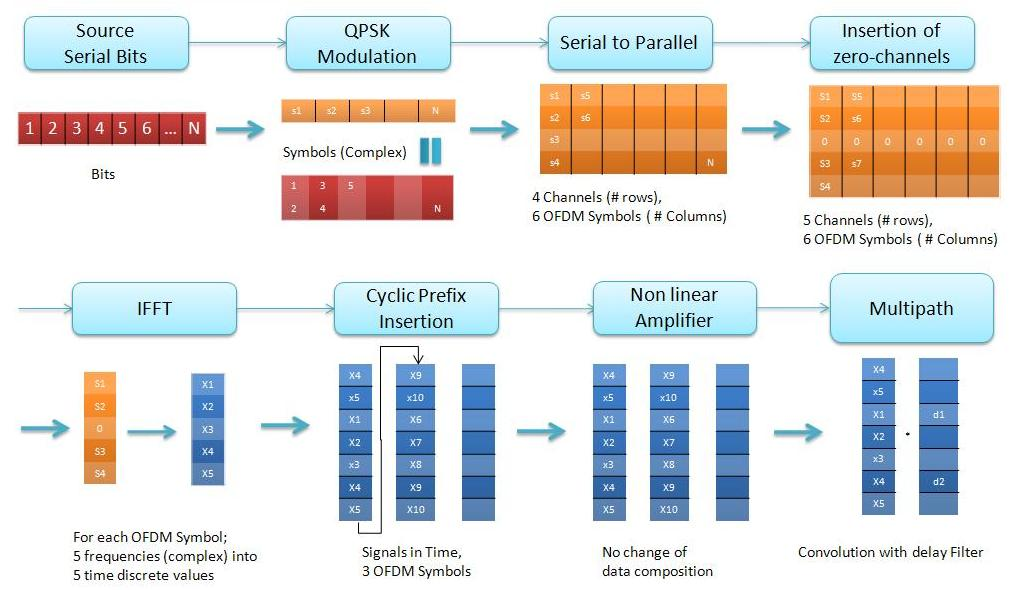
\includegraphics[width=\textwidth]{content/fig6/ofdmmodel1.JPG}
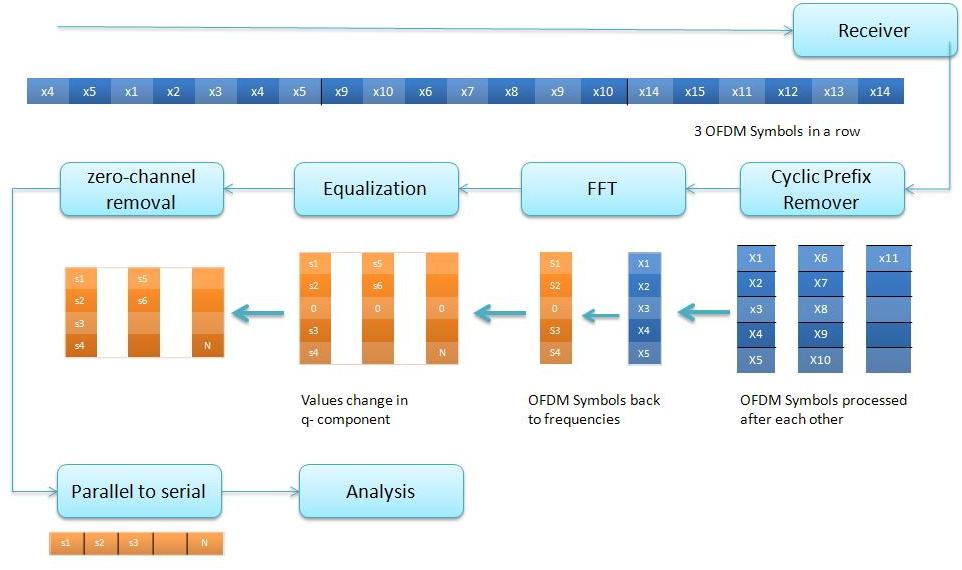
\includegraphics[width=\textwidth]{content/fig6/ofdmmodel2.JPG}
\caption{OFDM System Model}
\label{fig_ofdmsystemmodel}
\end{figure}

Figure \ref{fig_ofdmsystemmodel} presents the OFDM system block diagram.
Basic steps of the praxis are realized in blocks in the simulation. Additionally is shown how the composition of data changes in the single steps of the system.\\
The first block represents the data source. They are the bits which an application may send. In the simulation it is realized by a random bit generator. The following QPSK modulation block converts this bits into symbols, which are complex numbers. Each symbol carries several bits. The third block is the first one actually relevant for OFDM. The serial symbol stream is converted into a channel and OFDM symbol structure. In the simulation it is represented in a matrix shape where the rows are different channels and each column is an OFDM symbol. This means that each OFDM symbol, formed by $c$ (\#channels) serial symbols (complex numbers), is distributed over the $c$ channels.\\
In the next step zero channels are added in order to separate well subsequent OFDM symbols. For the simulation structure zero rows are added in the middle of the matrix. The following block interprets each symbol (complex number) of an OFDM symbol as a orthogonal frequency and converts each OFDM symbol per IFFT into a vector of time discrete values of the same length. As sixth step the cyclic prefix insertion is done. In order to maintain orthogonality of the frequencies but prevent ISI, an amount of \textit{guard values} are copied from the end of each OFDM symbol to its beginning. The number of rows in the simulation matrix grows by that by the number of \textit{guard values}.\\
The following block is the NLA which depends on the optimization parameter $\beta$ (back-off). At this point the transmitter side ends. In order to simulate the multipath a convolution is made on each OFDM symbol with the delay filter. Since the simulation is made on each OFDM symbol separated, this operation works with a memory in order simulate a serial transmission.\\
The receiver side is just the opposite of the transmitter. In the cyclic prefix remover the copied values are deleted and the simulation matrix size decreases. The next block performs the FFT on each OFDM symbol which reconstructs the as frequencies interpreted complex numbers.\\ The following equalization block tries to remove the effect of the multipath. For the simulation a multiplication with the inverted transfer function of the multipath is operated. By this, only the phase of the complex symbols changes.\\ Finally, the zero channels are removed and the matrix structure is reconverted to a series of symbols. The following analysis is done on the received symbols and consequently they are not demodulated into a bitstream.

\section{Simulation Structure}
\label{sec_simstruct}
Fundamentally, we do block-by-block simulation thanks to IFFT for parallel processing. Simulation is done by (de)activation of the blocks on Figure \ref{fig_ofdmsystemmodel}.
First, we study the noise semi-analysis by having only the basic blocks activated and also to examine the correctness of them. The basic blocks for our OFDM system are IFFT and FFT, Cyclic addition and removal and the semi-analyzer block. 
The theoretical equation of the BER for a QPSK channel is:\\
\begin{center} 
$P_{b}(e)= \frac{1}{2}erfc(\sqrt{\frac{E_{b}}{N_{0}}})$\\
\end{center}
It is discussed that the BER can be computed by considering the non-ideality which the two parameters \textit{guard time} and \textit{pilots} will inject into the result. The formulation would be:\\
\begin{center}
 $P_{b}(e)= \frac{1}{2}erfc(\sqrt{\frac{E_{b}}{N_{0}}\frac{T}{T+T_{g}}\frac{N_{u}}{N_{u}+N_{p}}})$\\
\end{center}

In the next step, the NLA block is activated and its effect is studied. We have chosen NLA number 3 and try to optimize its back-off.
Later, the channel impulse response modeled by considering two multipaths with different delays is implemented by an FIR filter. This extended simulation will be compared with NLA in the scenario and also the equalizer. Finally, we optimize the system by adjusting the back-off parameter of NLA in an AWGN channel.\\
When we study the equalization block we consider such equation for the received tones:
\begin{center}
$y_{i}= H_{i} \lambda_{i} + n_{i}$\\
\end{center}
Without equalization the BER would be:
\begin{center}
$P_{b}(e)= \frac{1}{2}erfc(\frac{H_{i} \lambda_{i}}{\sqrt{2 \sigma^{2}}})$\\
\end{center}
Then, after the equalization, the formula will be changed to this:\\
\begin{center}
$y^{\prime}_{i}= \lambda_{i} + \frac{n_{i}}{H_{i}}$\\
\end{center}
and the BER to
\begin{center}
 $P_{b}(e)= \frac{1}{2}erfc(\frac{\lambda_{i}}{\sqrt{2 \sigma^{2}}})$\\
\end{center}
and NOT: $P_{b}(e)= \frac{1}{2}erfc(\frac{\lambda_{i}}{\sqrt{\frac{2 \sigma^{2}}{H_{i}}}})$, as it may be guessed wrongly. The power spectral density of the noise is not decreased.
\section{System Design in System Generator}
\label{sec_anasim}

\begin{center}
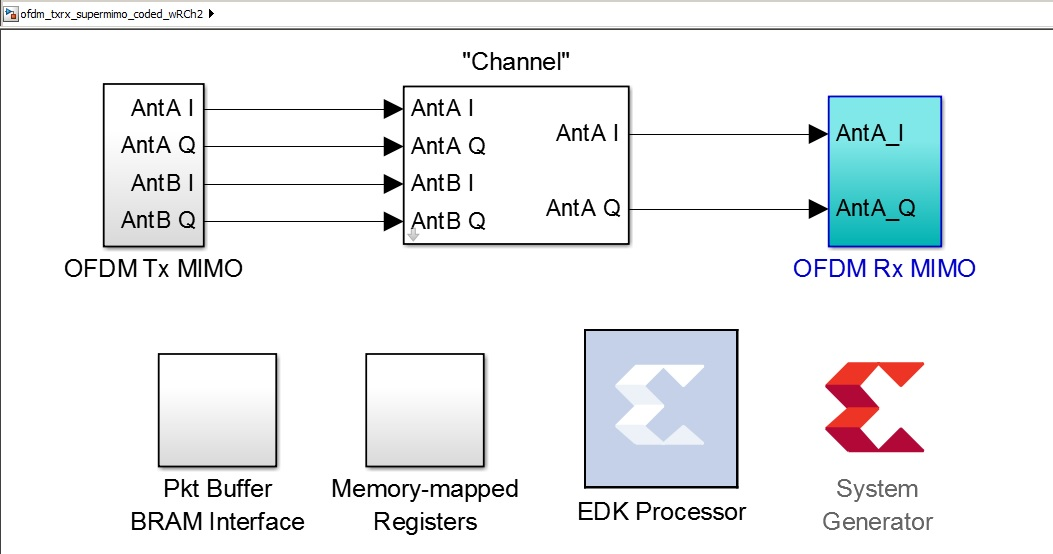
\includegraphics[width=\textwidth]{content/fig/system.JPG}
\captionof{figure}{OFDM System.}
\label{ofdm_system}
\end{center}


\begin{center}
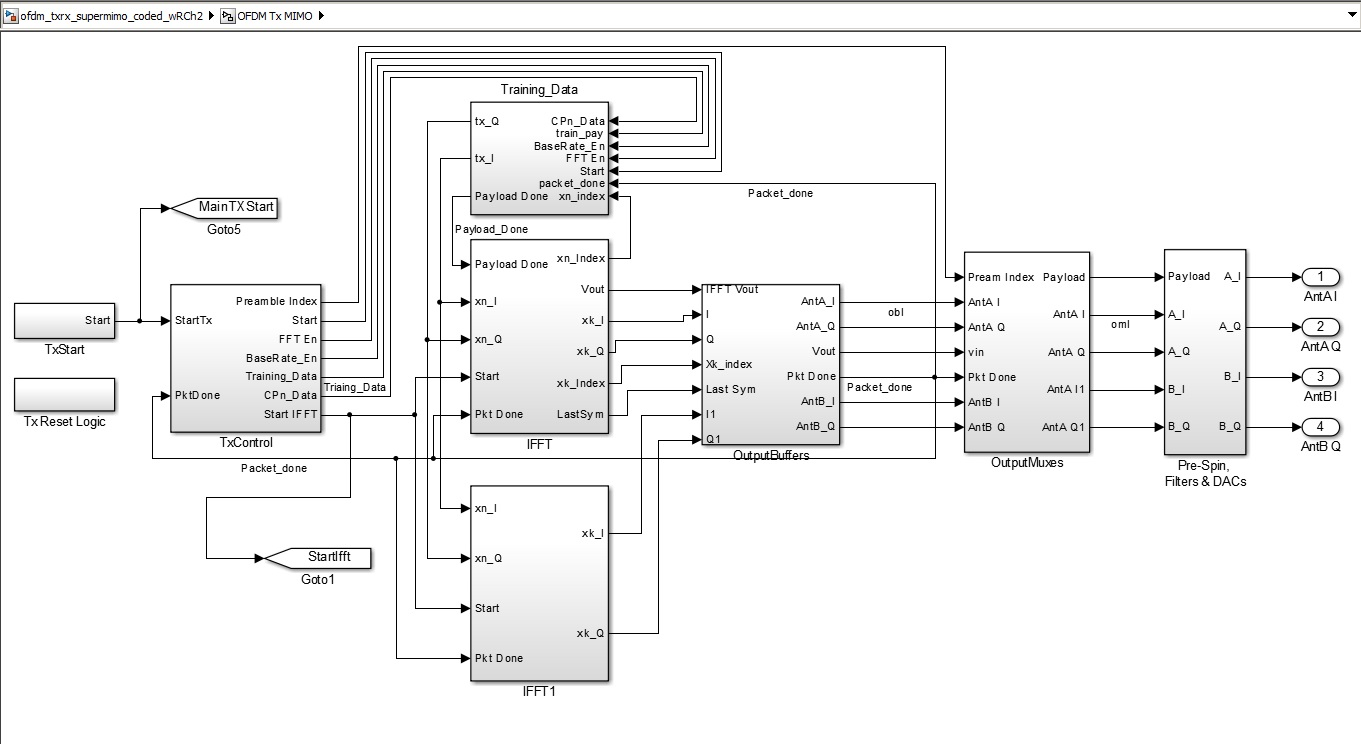
\includegraphics[width=\textwidth]{content/fig/txblock.JPG}
\captionof{figure}{OFDM Transmitter Block.}
\label{tx_block}
\end{center}

\begin{center}
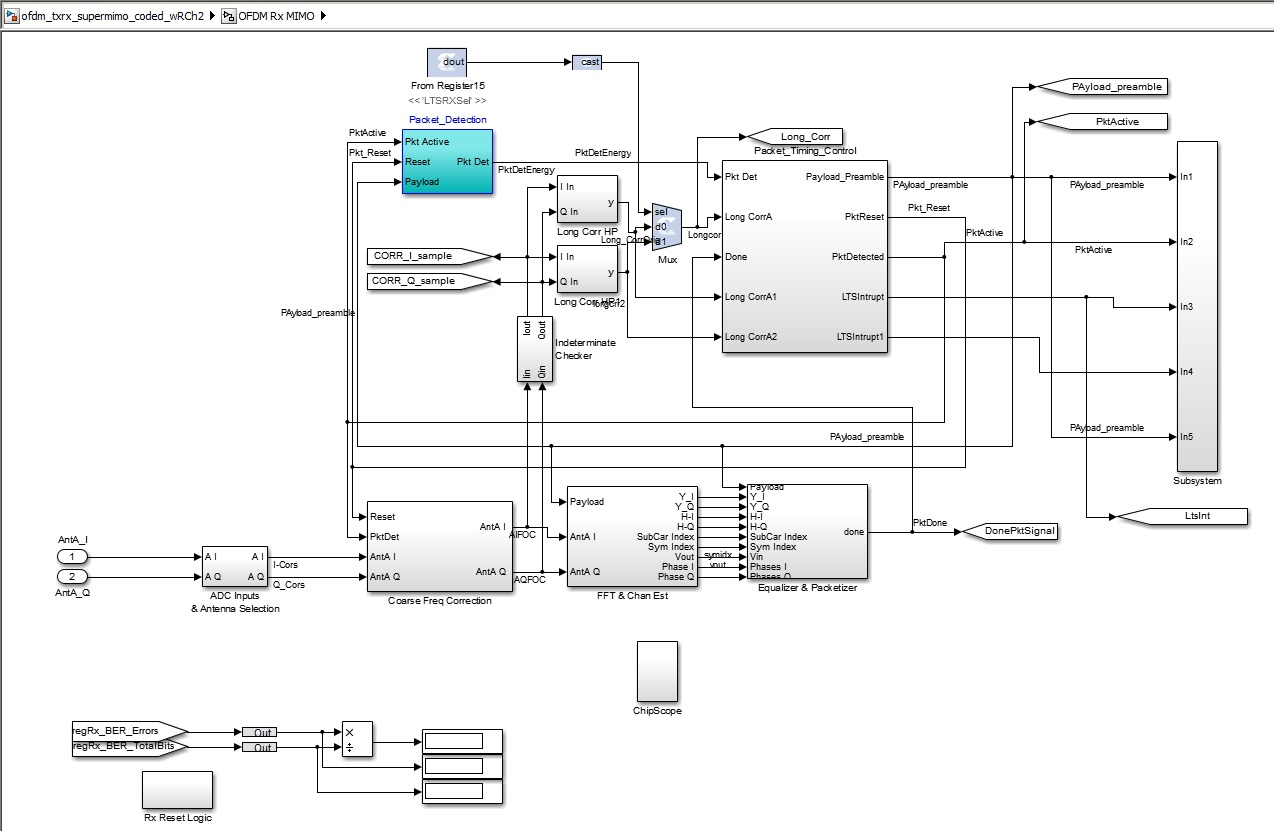
\includegraphics[width=\textwidth]{content/fig/rxblock.JPG}
\captionof{figure}{OFDM Receiver Block.}
\label{rx_block}
\end{center}

\begin{center}
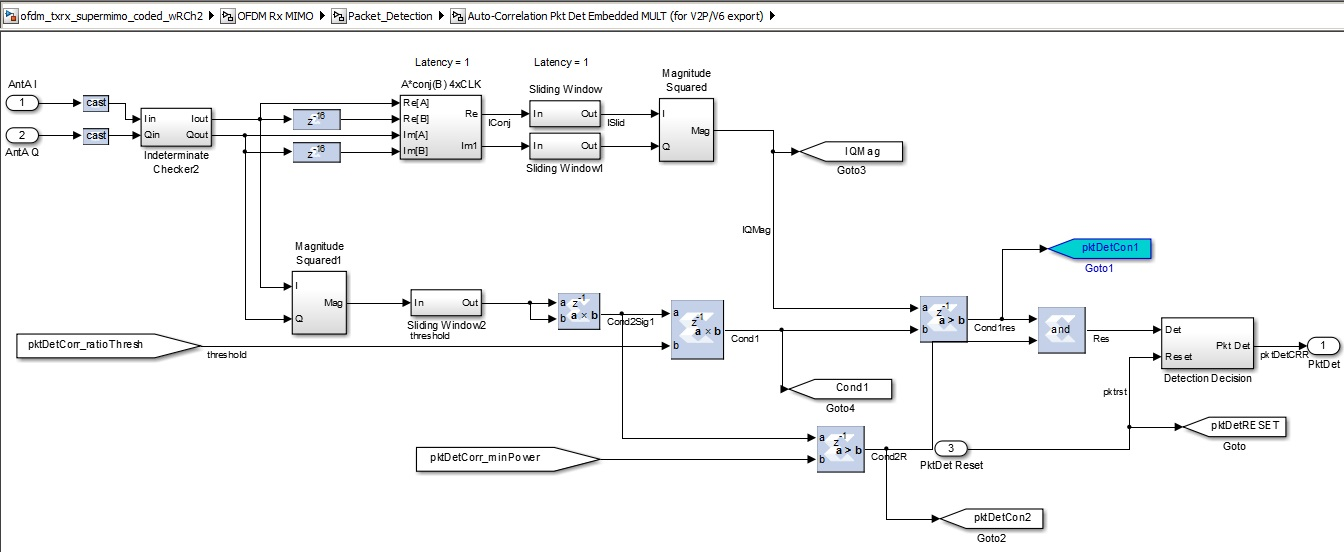
\includegraphics[width=\textwidth]{content/fig/autocorrblock.JPG}
\captionof{figure}{Auto-Correlation Block.}
\label{autocorrblock}
\end{center}

\begin{center}
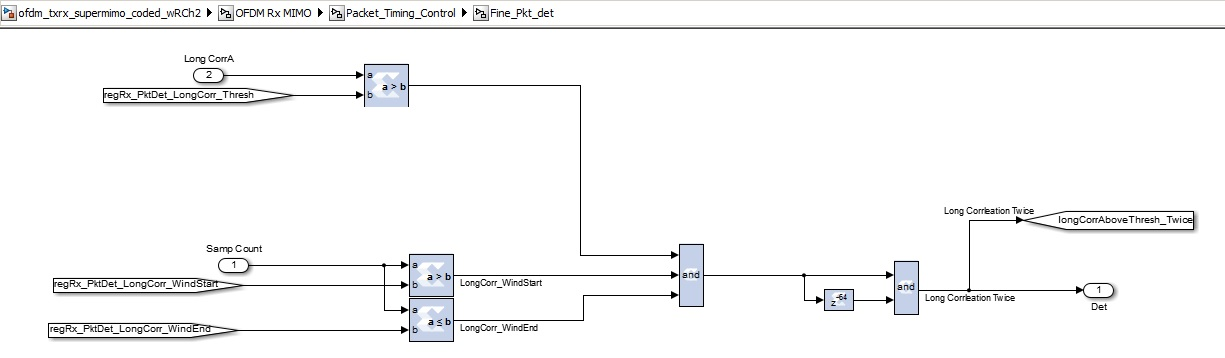
\includegraphics[width=\textwidth]{content/fig/fine_packetDetect.JPG}
\captionof{figure}{Fine Packet Detection Block.}
\label{autocorrblock}
\end{center}

\section{Hardware Samples and Analysis}
\label{hw_samples}

\begin{center}
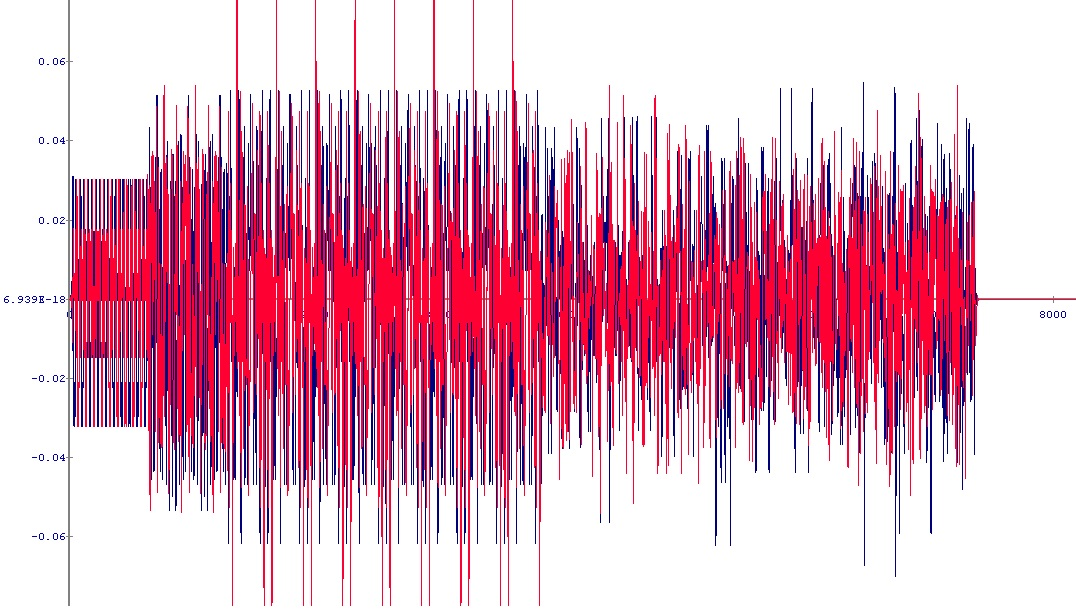
\includegraphics[width=\textwidth]{content/fig/ofdmframe_chipscope.JPG}
\captionof{figure}{OFDM Frame (I/Q) detected in Chipscope.}
\label{ofdmframe_chipscope}
\end{center}

\begin{center}
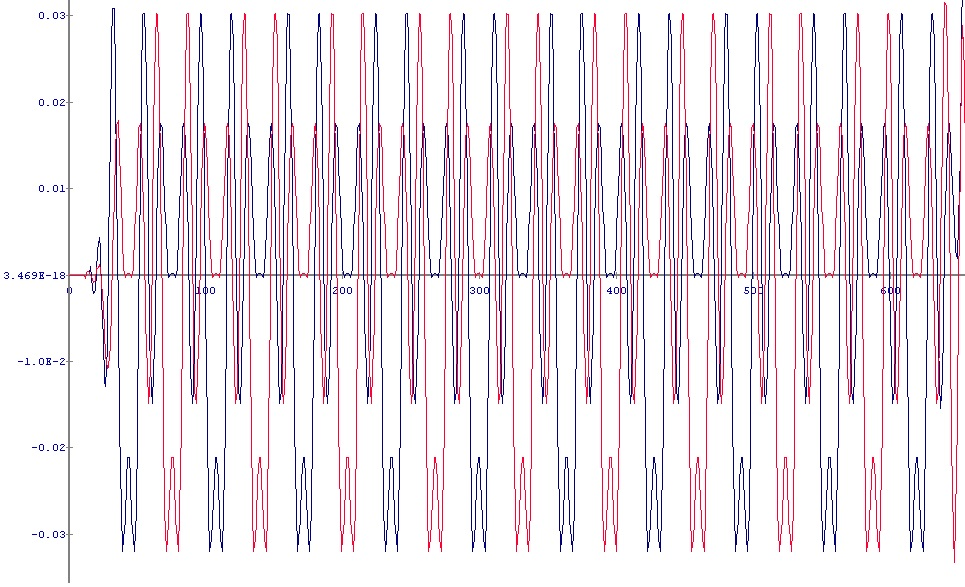
\includegraphics[width=\textwidth]{content/fig/sts_chipscope.JPG}
\captionof{figure}{STS (I/Q) detected in Chipscope.}
\label{sts_chipscope}
\end{center}

\begin{center}
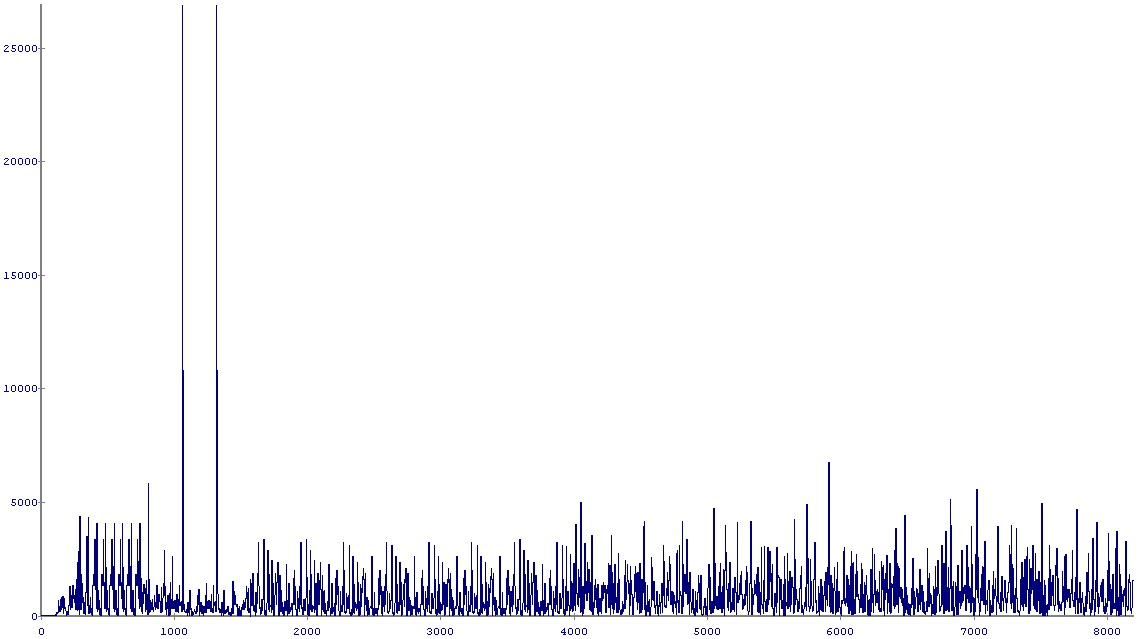
\includegraphics[width=\textwidth]{content/fig/crosscorr.JPG}
\captionof{figure}{Cross-Correlation detected in Chipscope.}
\label{crosscorr}
\end{center}


\begin{center}
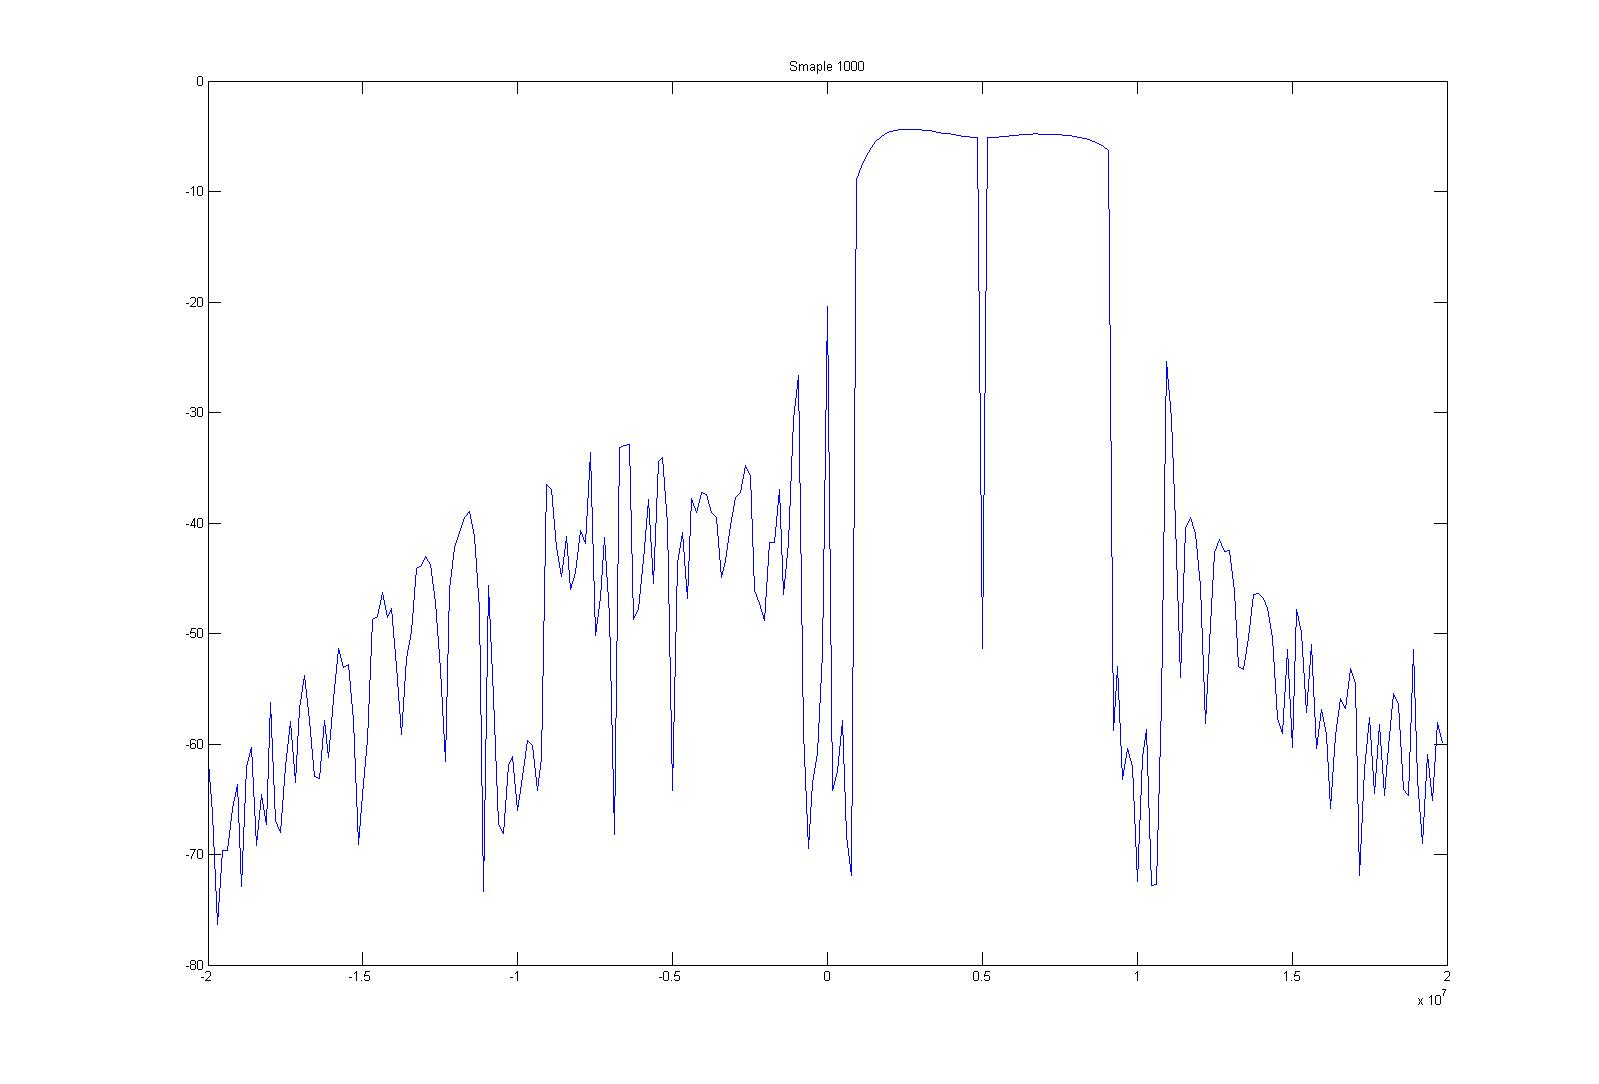
\includegraphics[width=\textwidth]{content/fig/baseIFAdcDac.JPG}
\captionof{figure}{LTS Spectrum in Baseband chain (IF filter is enable)}
\label{baseIFAdcDac}
\end{center}

\begin{center}
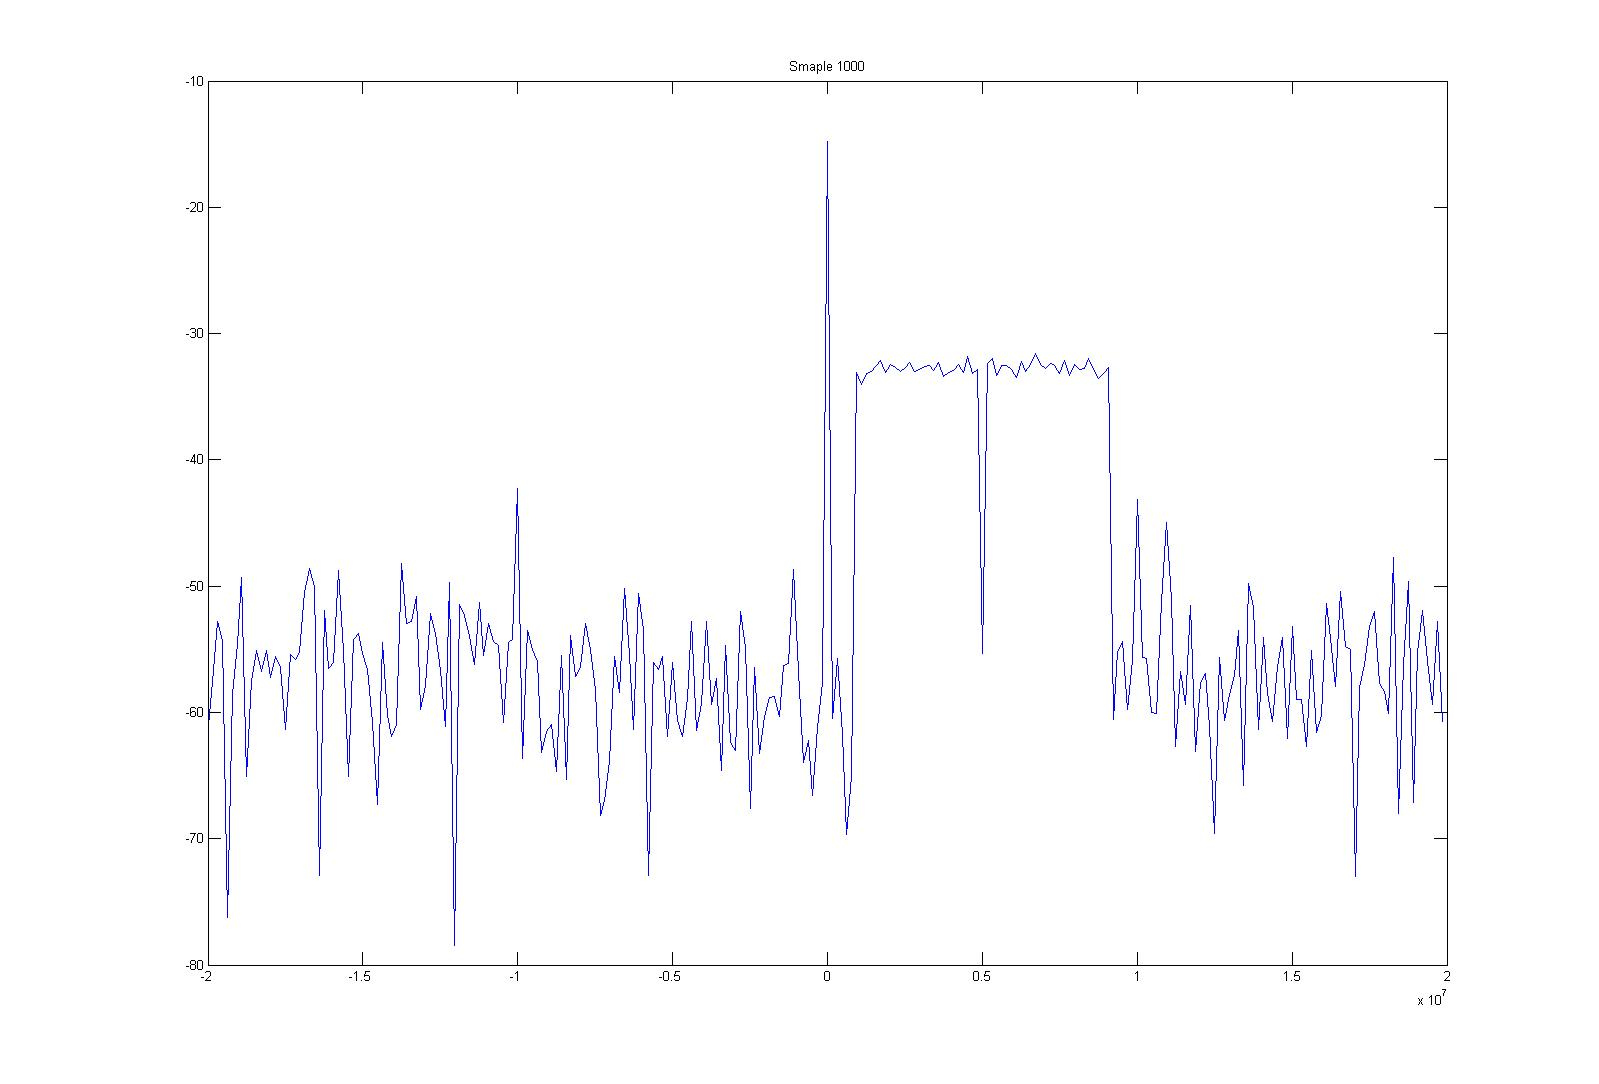
\includegraphics[width=\textwidth]{content/fig/RfIF.JPG}
\captionof{figure}{LTS Spectrum- passed RF chain (IF filter is enable)}
\label{RfIF}
\end{center}

\begin{center}
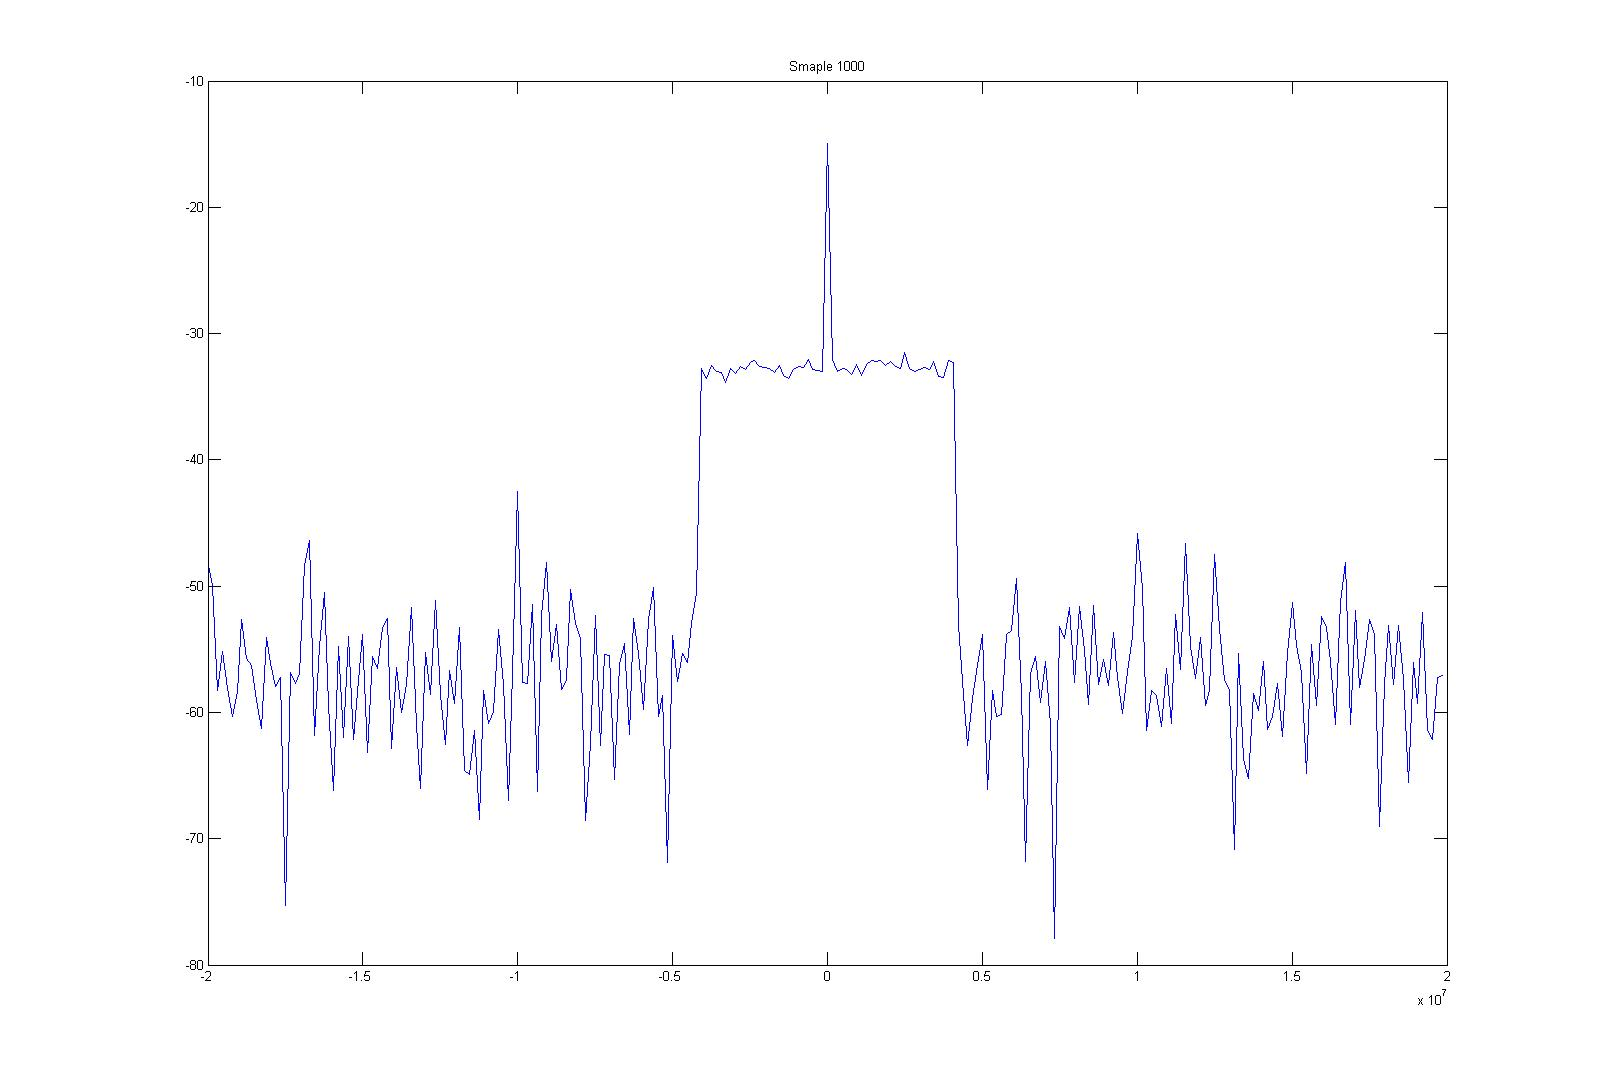
\includegraphics[width=\textwidth]{content/fig/Rfbase.JPG}
\captionof{figure}{LTS Spectrum- passed RF chain (IF filter is disable)}
\label{Rfbase}
\end{center}

\begin{center}
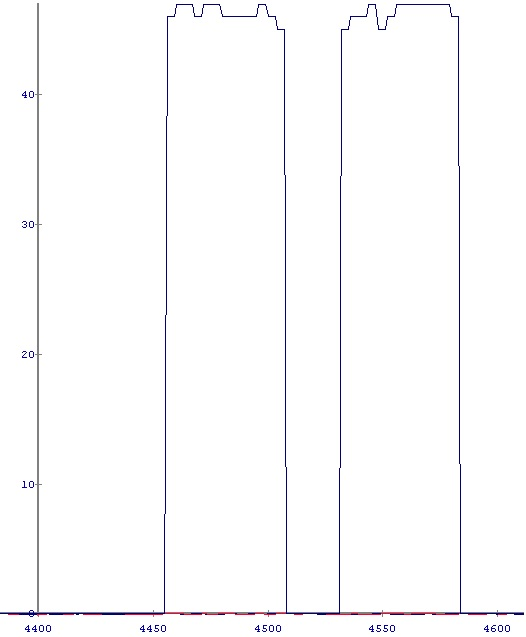
\includegraphics[width=\textwidth]{content/fig/h_mag_chipscope.JPG}
\captionof{figure}{Frequency Response of a semi-perfect channel}
\label{h_mag_chipscope}
\end{center}